\chapter{Results and Analysis}\label{ch:results}
% fluent: step, value, low, high
\def\bktfluent{(0,0.200) (1,0.586) (2,0.881) (3,0.974) (4,0.995) (5,0.999)}
\def\bktfluentlow{(0,0.200) (1,0.338) (2,0.678) (3,0.799) (4,0.838) (5,0.856)}
\def\bktfluenthigh{(0,0.200) (1,0.833) (2,1.000) (3,1.000) (4,1.000) (5,1.000)}
% recovering: step, value, low, high
\def\bktrecovering{(0,0.200) (1,0.157) (2,0.144) (3,0.356) (4,0.748) (5,0.939)}
\def\bktrecoveringlow{(0,0.200) (1,0.000) (2,0.000) (3,0.161) (4,0.577) (5,0.785)}
\def\bktrecoveringhigh{(0,0.200) (1,0.418) (2,0.361) (3,0.552) (4,0.919) (5,1.000)}
% struggling: step, value, low, high
\def\bktstruggling{(0,0.200) (1,0.157) (2,0.144) (3,0.139) (4,0.138) (5,0.137)}
\def\bktstrugglinglow{(0,0.200) (1,0.000) (2,0.000) (3,0.000) (4,0.000) (5,0.000)}
\def\bktstrugglinghigh{(0,0.200) (1,0.418) (2,0.361) (3,0.329) (4,0.309) (5,0.294)}

\def\topiclabels{{Basics},{Variables/IO},{Conditionals},{Loops},{Functions},{Strings},{Lists/dicts},{Recursion},{Search/sort},{Arrays},{Hashing},{Stacks/queues},{Linked lists},{Trees},{Graphs},{DP},{Toolkit}}
\def\topiceasy{(0,19) (1,18) (2,18) (3,20) (4,14) (5,28) (6,23) (7,10) (8,9) (9,13) (10,15) (11,6) (12,8) (13,14) (14,9) (15,6) (16,7)}
\def\topicmedium{(0,0) (1,4) (2,8) (3,12) (4,12) (5,9) (6,12) (7,12) (8,19) (9,19) (10,14) (11,15) (12,16) (13,17) (14,15) (15,21) (16,13)}
\def\topichard{(0,0) (1,0) (2,0) (3,0) (4,1) (5,0) (6,1) (7,5) (8,4) (9,5) (10,2) (11,8) (12,2) (13,0) (14,5) (15,7) (16,1)}

\def\catlabels{{efficiency check},{large input},{empty input},{large number},{all the same},{one},{reverse sorted},{repeated values},{negative numbers},{zero},{sorted},{single item},{typical}}
\def\catcoords{(7,0) (46,1) (394,2) (406,3) (552,4) (626,5) (634,6) (827,7) (850,8) (967,9) (1258,10) (2136,11) (6014,12)}

\def\auditlabels{{Checks over every hint shown},{Planner route and agreement},{Reflection question and reply},{Help offered, not pushed},{High mastery, overload, no history},{Return inside a loop},{Progress, new issue, solve},{Runtime error and endless loop},{Repeated syntax error},{Repeated requests on unchanged code}}
\def\auditcoords{(2,0) (3,1) (6,2) (3,3) (5,4) (2,5) (5,6) (3,7) (3,8) (7,9)}


\section{Evaluation setup}
In this phase we evaluated whether the system is correct, is safe and behaves as designed. We did not measure learning gains, because no study with real learners has been carried out yet. The planned study is described in Chapter~7.

All runs used the development machine described in Chapter~4 (Apple M2, 8~GB, macOS 27.2, Docker Desktop 29.8, Python 3.12.13, Node.js 26.4.0) with PostgreSQL 16.15 in a container. Every test used the real database, the real execution service with Docker sandbox containers, the real LangGraph pipeline and ChromaDB. No LLM was configured (\code{LLM\_PROVIDER=none}), so every hint, question and reply used the built-in, evidence-based wording. The LLM path was tested with a scripted stand-in model.

The evaluation had four parts.
\begin{itemize}
\item We ran four automated test suites against the code: the backend suite (pytest), the frontend unit suite (Vitest), the browser end-to-end suite (Playwright with Google Chrome and axe-core) and the execution-service suite. For the browser tests, a separate API and web server were started on other ports with raised rate limits, so that test traffic did not affect the developers' server.
\item We ran an agent audit. The script \code{scripts/agent\_audit.py} registers a fresh learner for each of nine scenarios, submits code or asks for hints on the problem ``Sum from 1 to N'', and reads each agent's output back from the run response and its per-stage trace. It checks 37 behavioural rules plus two rules over every hint shown.
\item We verified the curriculum. Every problem's reference solution was run against all of its tests in the sandbox, and every starter program was confirmed to fail.
\item We inspected the interface. The screenshots were captured by a script that drives the running application as a demo learner and a demo teacher.
\end{itemize}

We took four precautions against invalid results.
\begin{itemize}
\item The suites were run one at a time. In an earlier run they were run in parallel, which overloaded Docker on the 8~GB machine and produced false failures.
\item The final runs were made after the last code change, and the counts reported here are from those runs.
\item The audit reads the agents' outputs from the stored traces and not from the code under test, so it checks what the agents actually produced.
\item All synthetic data (the teacher demo class and the demonstration retrieval records) is labelled in the interface, and we do not use it as evidence that the tutor works.
\end{itemize}

\section{Evaluation criteria}
Table~\ref{tab:criteria} defines the criteria used.

\begingroup\small
\setlength{\tabcolsep}{4pt}\renewcommand{\arraystretch}{1.15}
\begin{longtable}{|R{3.4cm}|R{6.6cm}|R{3.6cm}|}
\caption{Evaluation criteria}\label{tab:criteria}\\\hline
\textbf{Criterion} & \textbf{Measure and interpretation} & \textbf{Target}\\\hline\endfirsthead
\hline\textbf{Criterion} & \textbf{Measure and interpretation} & \textbf{Target}\\\hline\endhead
Functional correctness & Tests passed $\div$ tests run, per suite. & 100\% on the final code.\\\hline
Agent behaviour & Audit checks passed $\div$ checks, over nine scenarios that exercise all six agents. & All checks pass.\\\hline
Non-repetition of help & Distinct hints among repeated requests on unchanged code; highest pairwise similarity $\operatorname{rep}(a,b)$ (Section~5.2). & All distinct; similarity $<0.8$.\\\hline
Controlled escalation & Level change between consecutive hints on one issue; hints shown without a request after a first hint. & At most $+1$; none shown unasked.\\\hline
Hint specificity & Share of hints that name a line, value or name from the learner's code, and share free of generic advice. & 100\% of hints shown.\\\hline
Solution protection & Responses containing hidden-test values or reference solutions; hints exceeding the solution-overlap threshold. & None.\\\hline
Curriculum validity & Problems whose reference solution passes all tests and whose starter fails. & All 496 problems.\\\hline
Test coverage & Tests per problem; share of problems with at least 30 tests. & Coverage reported.\\\hline
Accessibility & Automated WCAG 2.0 and 2.1 A and AA violations on main screens, both themes. & Zero violations.\\\hline
\end{longtable}
\endgroup

\section{Result}
\subsection{Automated test suites}
Table~\ref{tab:tests} summarises the final runs. Every suite passed in full.

\begin{table}[htbp]\centering\small
\caption{Results of the automated test suites on the final code}\label{tab:tests}
\begin{tabular}{|R{3.6cm}|R{2.2cm}|R{7.6cm}|}\hline
\textbf{Suite} & \textbf{Result} & \textbf{What it exercises}\\\hline
Backend (pytest) & 551 of 551 & API, all six agents, the full pipeline, persistence, retrieval, policy, hint quality, imports and content, with real PostgreSQL, sandbox, LangGraph and ChromaDB.\\\hline
Browser end-to-end (Playwright) & 59 of 59 & 54 learner and teacher flows in real Chrome, and 5 automated accessibility tests in light and dark themes.\\\hline
Frontend unit (Vitest) & 21 of 21 & Shared interface components, draft restoration, test-case editing, display formatting, saved-data migration and new-tab links.\\\hline
Execution service & 39 of 39 & 26 execution tests and 13 isolation tests in real containers (run on 9 November 2026; this service did not change afterwards).\\\hline
Agent audit & 37 of 37, plus 2 of 2 & Nine scenarios through the running stack; two further checks over all 17 hints shown.\\\hline
Curriculum verification & 496 of 496 & Each reference solution passes all of its tests (15,717 in total) and each starter fails, in the sandbox.\\\hline
Static checks & Passed & Ruff lint (backend), TypeScript strict type check and production build (frontend).\\\hline
\end{tabular}
\end{table}

Figure~\ref{fig:backend-tests} shows how the 551 backend tests are spread across the test files. The largest file covers repeated-hint behaviour, which is where we found the most serious defect during development (Section~\ref{sec:compare}).

\begin{figure}[htbp]\centering
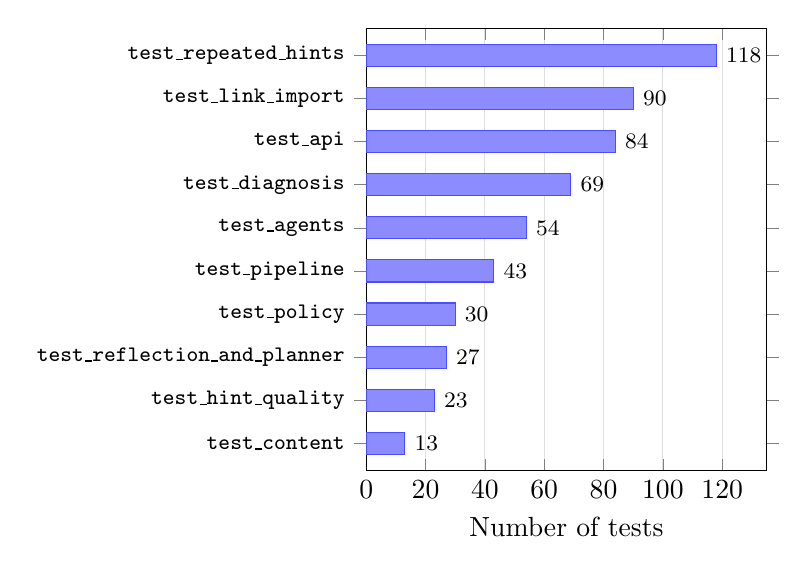
\begin{tikzpicture}
\begin{axis}[xbar, width=0.55\textwidth, height=7.2cm, xmin=0, xmax=135, bar width=8pt,
  ytick={0,...,9}, yticklabels={{test\_content},{test\_hint\_quality},{test\_reflection\_and\_planner},{test\_policy},{test\_pipeline},{test\_agents},{test\_diagnosis},{test\_api},{test\_link\_import},{test\_repeated\_hints}},
  yticklabel style={font=\footnotesize\ttfamily}, xlabel={Number of tests}, nodes near coords, nodes near coords style={font=\footnotesize},
  enlarge y limits=0.07, xmajorgrids, grid style={gray!25}]
\addplot[fill=blue!45, draw=blue!70] coordinates {(13,0) (23,1) (27,2) (30,3) (43,4) (54,5) (69,6) (84,7) (90,8) (118,9)};
\end{axis}
\end{tikzpicture}
\caption{Backend tests per test file (551 in total, all passed)}\label{fig:backend-tests}
\end{figure}

\subsection{Agent audit}
In the final audit run all 37 behavioural checks passed, and so did both checks over every hint (Figure~\ref{fig:audit}). Table~\ref{tab:audit} lists representative checks with the evidence the audit recorded.

\begin{figure}[htbp]\centering
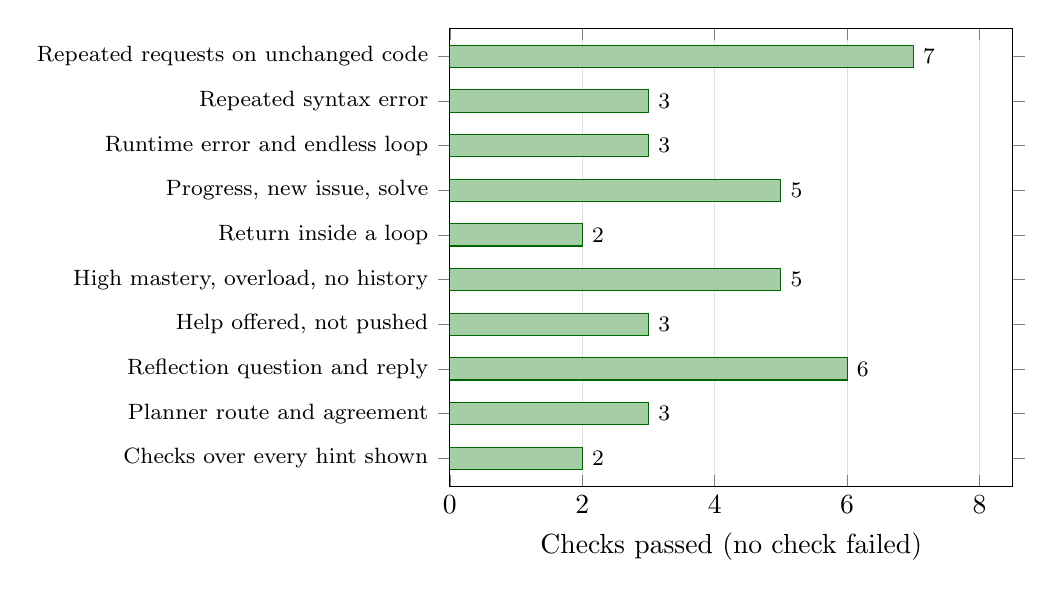
\begin{tikzpicture}
\begin{axis}[xbar, width=0.72\textwidth, height=7.4cm, xmin=0, xmax=8.5, bar width=8pt,
  ytick={0,...,9}, yticklabels/.expanded={\auditlabels}, yticklabel style={font=\footnotesize},
  xlabel={Checks passed (no check failed)}, nodes near coords, nodes near coords style={font=\footnotesize},
  enlarge y limits=0.07, xmajorgrids, grid style={gray!25}, xtick={0,2,4,6,8}]
\addplot[fill=green!45!black!35, draw=green!40!black] coordinates {\auditcoords};
\end{axis}
\end{tikzpicture}
\caption{Agent audit: checks passed per scenario (39 of 39)}\label{fig:audit}
\end{figure}

\begingroup\small
\setlength{\tabcolsep}{4pt}\renewcommand{\arraystretch}{1.15}
\begin{longtable}{|R{5.2cm}|R{8.4cm}|}
\caption{Representative audit checks and recorded evidence}\label{tab:audit}\\\hline
\textbf{Check} & \textbf{Evidence recorded in the final run}\\\hline\endfirsthead
\hline\textbf{Check} & \textbf{Evidence recorded in the final run}\\\hline\endhead
Every request on unchanged code gets a different hint & 4 requests, 4 different hints; pairwise similarities 0.16 to 0.38 (all below 0.8).\\\hline
Escalation is gradual & Levels 2, 2, 2, 3; strategies targeted hint, trace the failing case, print debugging, step outline.\\\hline
Retrieval leaves out approaches already shown & Excluded strategies grew with each request: none; targeted hint; then also trace; then also print debugging.\\\hline
Syntax error is diagnosed with its line & \code{SyntaxError: expected ':'}; first hint: ``Look at line 1. A line that opens a block \ldots{} must end with one particular punctuation mark. Which mark is missing there?''\\\hline
Runtime cause is told apart from a generic error & \code{UnboundLocalError} diagnosed as ``used before assignment'', confidence 0.95.\\\hline
Endless loop is diagnosed as a timeout & \code{timeout:loop\_no\_progress}; the hint asks the learner to follow \code{while i <= n:} on line 4 by hand.\\\hline
Help is offered, not pushed & First failed submission: a hint. Next two failed submissions: \code{offer\_help} both times. Asking then: next step, level 2.\\\hline
Overloaded learner & One short action of 33 words and no reflection question (deferred).\\\hline
Unknown stays unknown & With no history, confusion is reported as unknown rather than assumed.\\\hline
Reflection holds back a plan that was moving on & After a first-try solve the plan was ``Count the Digits'' (next technique); the answer ``not sure, I just changed it until it passed'' changed it to ``Sum Odds Only'' (one more running-totals problem).\\\hline
Reflection does not repeat the plan & After a solve with help the plan already gave one more running-totals problem; the same unsure answer left it unchanged.\\\hline
Planner moves forward & Route: Loops, Functions, Strings, Lists and dictionaries; the home screen suggested the same next problem as the plan.\\\hline
Every hint is specific & All 17 hints shown named a line, value or name from the learner's code, and none used generic advice such as ``check your logic''.\\\hline
\end{longtable}
\endgroup

\subsection{Tutoring behaviour in the interface}
Figures~\ref{fig:hint} to~\ref{fig:route} show one learner session on ``Sum from 1 to N'', captured from the running application. The code loops over \code{range(1, n)}, so it misses the last value.

\screenshot{workspace_first_hint.png}{First wrong submission: the tutor gives one targeted hint built from the learner's own failing call, values and loop variable, with the concept, a link to the lesson and a ``Why this hint?'' explanation}{fig:hint}

\screenshot{offer_not_pushed.png}{Second wrong submission on the same issue: the next hint is offered, not shown, and says once what it will focus on}{fig:offer}

\screenshot{reflection_reply.png}{After three failed attempts: a reflection question about the learner's own loop, and the tutor's reply to the answer ``no idea''}{fig:reflection}

\screenshot{solved_plan_route.png}{After the solve: a question about the technique, and a next step on the same technique without hints, with the route ahead}{fig:solved}

\screenshot{home_route.png}{Home screen after the session: the same next step as the plan, with the route through the course}{fig:route}

\screenshot{teacher_dashboard.png}{Teacher dashboard with the clearly labelled synthetic demonstration class; the numbers are generated and are not evidence that the tutor works}{fig:teacher}

\subsection{Learner-state estimates}
Figure~\ref{fig:bkt} shows how the implemented mastery update responds to three attempt sequences. We computed the curves by running the Cognitive State agent's own functions with its configured parameters. A learner who solves five times without help rises quickly. A learner who fails twice, solves once with a level-2 hint and then solves twice alone drops first and then recovers. A learner who keeps failing stays low. The dotted lines mark the band boundaries, and the band stays ``not enough evidence'' until the total evidence weight reaches 1.5. These curves come from the model alone and illustrate its behaviour. No data from real learners is involved.

\begin{figure}[htbp]\centering
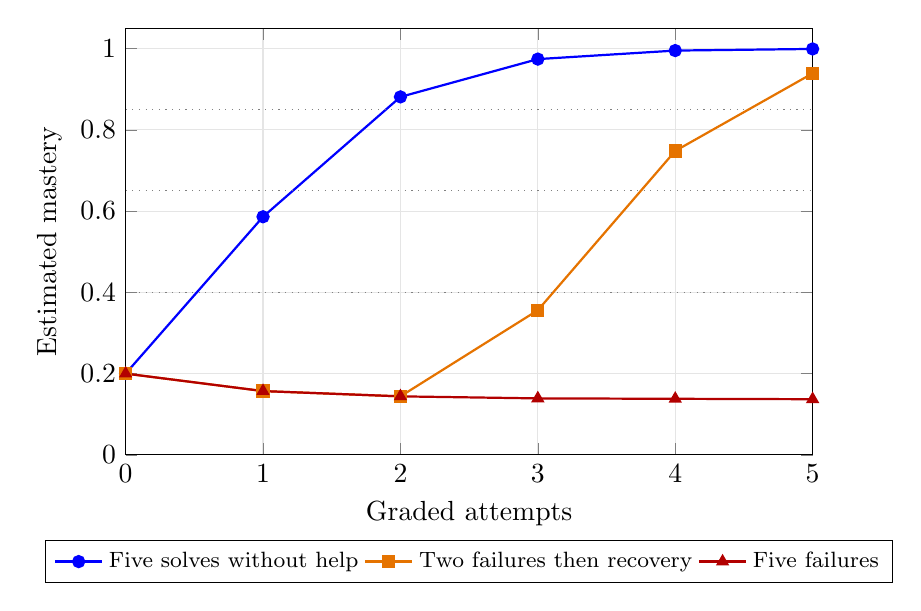
\begin{tikzpicture}
\begin{axis}[width=0.85\textwidth, height=7cm, xmin=0, xmax=5, ymin=0, ymax=1.05, xtick={0,...,5}, xlabel={Graded attempts}, ylabel={Estimated mastery},
  legend style={at={(0.5,-0.2)}, anchor=north, legend columns=3, font=\footnotesize}, grid=major, grid style={gray!20}]
\addplot[thick, blue, mark=*] coordinates {\bktfluent};
\addplot[thick, orange!90!black, mark=square*] coordinates {\bktrecovering};
\addplot[thick, red!70!black, mark=triangle*] coordinates {\bktstruggling};
\addplot[dotted, gray, domain=0:5] {0.40};
\addplot[dotted, gray, domain=0:5] {0.65};
\addplot[dotted, gray, domain=0:5] {0.85};
\legend{Five solves without help, Two failures then recovery, Five failures}
\end{axis}
\end{tikzpicture}
\caption{Mastery estimates produced by the implemented weighted knowledge-tracing update for three attempt sequences}\label{fig:bkt}
\end{figure}

\subsection{Curriculum and tests}
The curriculum has 496 verified problems in 17 topics (Figure~\ref{fig:curriculum}). The earlier topics are mostly easy, and the later data-structure topics are mostly medium and hard. Of the 15,717 tests, 1,000 are visible and 14,717 are hidden. In all, 487 problems have at least 30 tests (median 32, maximum 34). The other nine have few possible inputs, for example a problem that takes no input. Hidden tests are chosen to cover different kinds of input (Figure~\ref{fig:categories}).

\begin{figure}[htbp]\centering
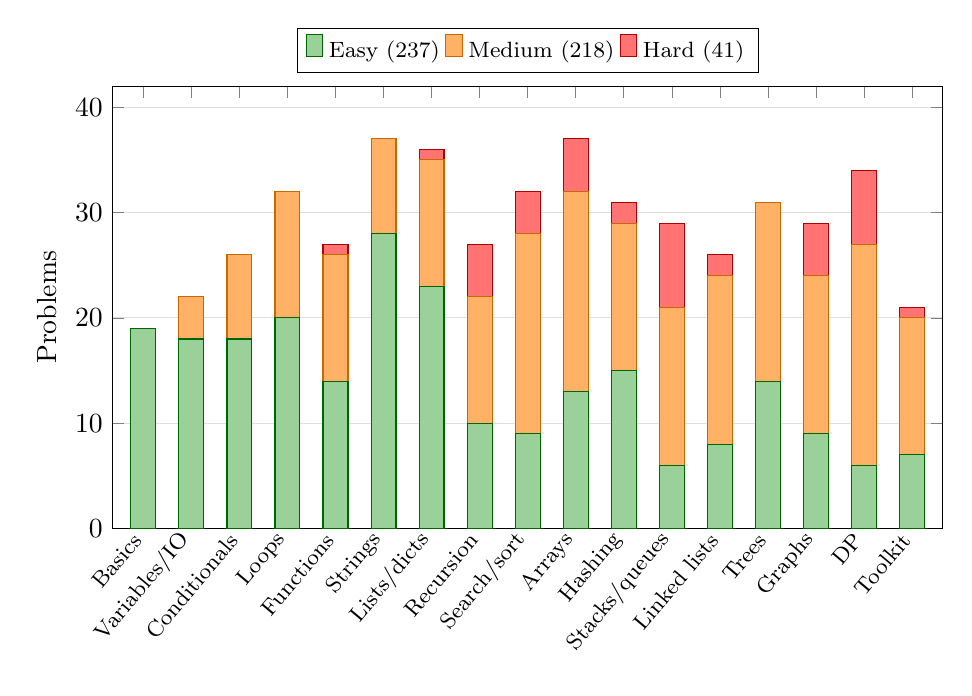
\begin{tikzpicture}
\begin{axis}[ybar stacked, width=\textwidth, height=7.2cm, bar width=9pt, ymin=0, ymax=42,
  xtick={0,...,16}, xticklabels/.expanded={\topiclabels}, xticklabel style={rotate=50, anchor=east, font=\footnotesize},
  ylabel={Problems}, legend style={at={(0.5,1.03)}, anchor=south, legend columns=3, font=\footnotesize}, ymajorgrids, grid style={gray!25}, enlarge x limits=0.04]
\addplot[fill=green!55!black!40, draw=green!40!black] coordinates {\topiceasy};
\addplot[fill=orange!60, draw=orange!80!black] coordinates {\topicmedium};
\addplot[fill=red!55, draw=red!70!black] coordinates {\topichard};
\legend{Easy (237), Medium (218), Hard (41)}
\end{axis}
\end{tikzpicture}
\caption{Curriculum problems per topic and difficulty (496 in total)}\label{fig:curriculum}
\end{figure}

\begin{figure}[htbp]\centering
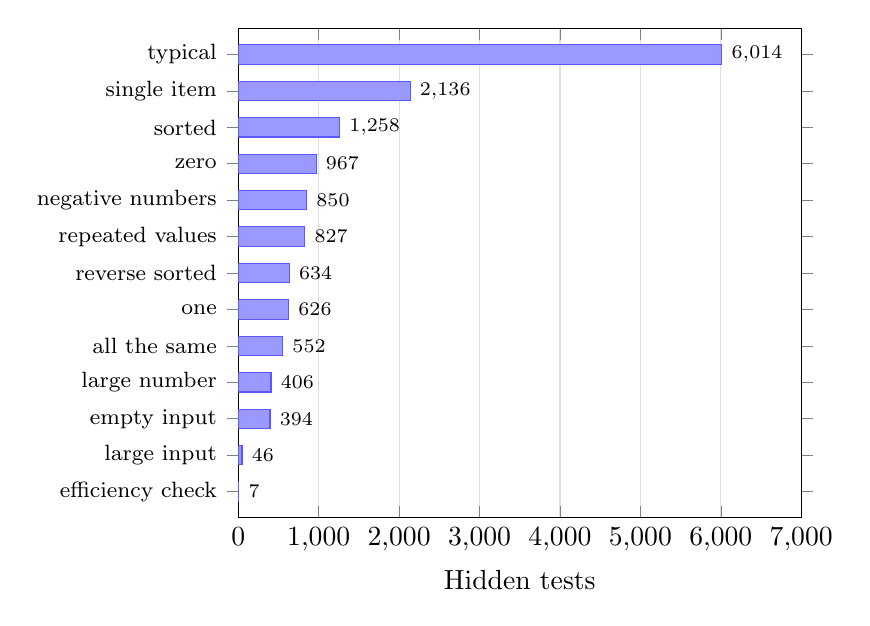
\begin{tikzpicture}
\begin{axis}[xbar, width=0.72\textwidth, height=7.8cm, xmin=0, xmax=7000, bar width=7pt,
  ytick={0,...,12}, yticklabels/.expanded={\catlabels}, yticklabel style={font=\footnotesize},
  xlabel={Hidden tests}, nodes near coords, nodes near coords style={font=\scriptsize},
  enlarge y limits=0.06, xmajorgrids, grid style={gray!25}, scaled x ticks=false]
\addplot[fill=blue!40, draw=blue!65] coordinates {\catcoords};
\end{axis}
\end{tikzpicture}
\caption{Hidden tests by kind of input (14,717 in total)}\label{fig:categories}
\end{figure}

\section{Comparative Analysis}\label{sec:compare}
\subsection{Before and after the agent improvements}
During development we reproduced the repeated-hint defect and recorded the behaviour before the fix, with five requests on unchanged code in each scenario. Table~\ref{tab:before-after} compares that behaviour with the final system.

\begingroup\small
\setlength{\tabcolsep}{4pt}\renewcommand{\arraystretch}{1.15}
\begin{longtable}{|R{3.7cm}|R{4.8cm}|R{5.1cm}|}
\caption{Behaviour before and after the agent improvements}\label{tab:before-after}\\\hline
\textbf{Behaviour} & \textbf{Before} & \textbf{After (final system)}\\\hline\endfirsthead
\hline\textbf{Behaviour} & \textbf{Before} & \textbf{After (final system)}\\\hline\endhead
Repeated hint requests on unchanged code & 1 distinct hint in 5 requests in every scenario (syntax, missing colon, off-by-one, runtime, timeout); constant level and support score 0.208 & 4 different hints in 4 requests, highest similarity 0.38; levels 2, 2, 2, 3; a different strategy each time; then the tutor waits for a code change\\\hline
Wrong submissions without asking & Each further failed submission on an issue could show the next, more revealing hint automatically & After a first hint, help is offered and shown only when asked, at most one level higher\\\hline
Reflection & Fixed questions, the same for every learner; answers stored with no reply and no effect & Questions name the learner's own code or technique; every answer gets a reply; an unsure answer reaches the Cognitive State and the Planner\\\hline
Planning & Next problem chosen by difficulty only; next topic could be an earlier topic with no work in it & Technique-by-technique sequencing at each difficulty; forward topic order; route shown; home screen and plan agree\\\hline
Hints for logic mistakes & 8 of 16 hints in the first audit run named nothing concrete from the learner's code & All 17 hints in the final run name a line, value or name from the learner's code\\\hline
\end{longtable}
\endgroup

\subsection{Comparison with existing approaches}
Table~\ref{tab:capability} compares what CodePath implements with what is described for the most closely related systems we reviewed. For the other systems, the entries state only what their published records describe, and ``Not reported'' does not mean that the system lacks the capability. The CodePath row lists functions that are implemented and tested. None of its entries is a measured learning effect.

\begin{landscape}
\begingroup\small
\setlength{\tabcolsep}{4pt}\renewcommand{\arraystretch}{1.2}
\begin{longtable}{|R{2.8cm}|R{3.2cm}|R{3.4cm}|R{3.0cm}|R{3.0cm}|R{2.7cm}|R{2.6cm}|}
\caption{Capabilities of CodePath and closely related systems}\label{tab:capability}\\\hline
\textbf{System} & \textbf{Persistent learner model} & \textbf{Decides how much help} & \textbf{Withholds full solutions} & \textbf{Retrieval} & \textbf{Several agents} & \textbf{Live programming practice}\\\hline\endfirsthead
\hline\textbf{System} & \textbf{Persistent learner model} & \textbf{Decides how much help} & \textbf{Withholds full solutions} & \textbf{Retrieval} & \textbf{Several agents} & \textbf{Live programming practice}\\\hline\endhead
Knowledge tracing \cite{corbett1995} & Yes (per skill) & Selects exercises until mastery & Not applicable & Not reported & Not reported & Yes\\\hline
CodeHelp \cite{liffiton2023} & Not reported & Not reported & Yes (guardrails) & Not reported & Not reported & Yes\\\hline
CodeAid \cite{kazemitabaar2024} & Not reported & Not reported & Yes & Not reported & Not reported & Yes\\\hline
PyTutor \cite{yang2024} & Not reported & Structured hint types & No (hints include coding solutions) & Not reported & Not reported & Yes\\\hline
RAGMan \cite{ma2024} & Not reported & Not reported & Not reported & Course material & Not reported & Yes\\\hline
Ruffle\&Riley \cite{schmucker2024} & Not reported & Not reported & Not applicable & Not reported & Yes (two agents) & No (biology)\\\hline
TRAVER \cite{wang2025} & Yes (knowledge tracing) & Not reported & Not reported & Not reported & Not reported & Simulated students\\\hline
\textbf{CodePath (this work)} & \textbf{Yes: mastery with range, confusion, load, progress} & \textbf{Yes: DSDA level, strategy and timing} & \textbf{Yes: validator and tests} & \textbf{Similar learners' outcomes} & \textbf{Yes: six agents} & \textbf{Yes}\\\hline
\end{longtable}
\endgroup
\end{landscape}

\subsection{Comparison with the proposal's evaluation metrics}
The initial submission proposed four evaluation measures: learning gain, hint efficiency and hints per problem, task completion rate and time to completion, and student satisfaction. All four are implemented as defined formulas in the teacher dashboard (Section~5.2), and tests cover their computation. We do not yet have their values for real learners. The only numbers shown at present come from the synthetic demonstration class (Figure~\ref{fig:teacher}) and are labelled as such. Learning gain is shown only for learners who have taken both knowledge checks, and this is intentional.

\section{Discussion and Interpretation}
Objective O1 (multiple collaborating agents) is met. Every learner action runs through six agents with typed contracts. The agents read each other's outputs and the stored history, and the pipeline tests and the audit confirm both the order and the data passed between them.

Objective O2 (cognitive state) is met in the form of explainable behavioural estimates. In the audit, confusion stays unknown without evidence and rises with repeated requests, and progress is detected when a new version gets further. We have not compared these estimates with any external measure of a learner's state, so they should be read as the tutor's working hypotheses.

Objective O3 (similar-learner retrieval) is met as a mechanism. Retrieval filters by similarity, outcome, difficulty and topic, excludes approaches already seen and refuses to answer on thin evidence. How useful it really is depends on outcomes from real learners, and those do not exist yet.

Objective O4 (scaffolding algorithm) is met. DSDA produces a level, a strategy and a timing with stated reasons, and the code reproduces its documented worked example exactly. The audit confirms the teaching behaviours we designed for: help does not repeat, rises at most one level at a time, is not pushed after a first hint, stays short for an overloaded learner and never contains a solution.

Objective O5 (effectiveness on datasets) is partly met. The curriculum dataset is verified, and so is the system's behaviour across realistic scenarios. Whether the tutor improves learning is not yet known.

The results also say something about \emph{how} help is given, which is where this project started. Table~\ref{tab:before-after} shows that the final system behaves much more like a patient human tutor than the earlier version did. It waits for the learner to try their own idea, gives one specific next step when asked, reacts to what the learner says in reflection, and moves forward through the course at a pace set by the learner's own work. The literature gives reasons for caution here. Help-seeking feedback can change behaviour without improving learning \cite{aleven2016}, and engaging tutors do not necessarily outperform reading \cite{schmucker2024}. The next phase therefore has to measure learning directly.

\section{Limitations}
\begin{itemize}
\item We have no evidence yet that the tutor improves learning. Real learners have not used the system, and every weight and threshold in the policy is a starting value chosen by judgement.
\item The estimates are behavioural. Confusion and load are inferred from behaviour and have not been validated against an external measure.
\item The similar-situation records are currently synthetic demonstration cases plus outcomes pooled from automated test and audit runs. The pooled outcomes count as ``live'' in the development database, so a fresh database is needed for any study.
\item No real model was tested. The available model key had no credit, so model-written wording, rejection rates and latency are unknown, and all the behaviour we observed used built-in wording.
\item Some checks are heuristic. The validator detects copied and lightly reworded solutions and repeats, but a determined rewording could pass. Reflection replies spot key ideas by keywords, so an unusual but correct answer can be read as partial.
\item Error-cause analysis covers common causes, and an unusual error falls back to general help with lower confidence. Built-in hints quote the learner's own code for ten common logic and timeout issues.
\item The sandbox was tested on Docker Desktop for macOS and not on a Linux server, and it has not been independently audited. The worker pool, queue and rate limits are held in memory, so the API runs as a single process.
\item Only Python is supported. The curriculum was written for this project and its difficulty labels are the authors' judgement. CodeNet was not imported.
\item Accessibility was checked automatically and not with screen-reader users, and the browser tests ran on Chrome only.
\end{itemize}
